\documentclass[12pt, letterpaper]{report}
\usepackage[utf8]{inputenc}
\usepackage{graphicx}
\usepackage{indentfirst}
\usepackage{url}
\usepackage{titling}

\graphicspath{{./images/}}

\newcommand{\subtitle}[1]{%
  \posttitle{%
    \par\end{center}
    \begin{center}\LARGE#1\end{center}
    \vskip0.5em}%
}

\title{\textbf{Smart Street Lighting}}

\subtitle{{\large Master in Industrial Eletronics and Computers Engeneering} \\ {\large Embedded Systems}}

\author{Authors:\\Diogo Fernandes PG47150\\José Tomás Abreu PG47386\\ \\ Supervisors:\\Prof. Dr. Tiago Gomes\\Prof. Ricardo Roriz\\Prof. Sérgio Pereira}

\date{\today}

\begin{document}

{\begin{figure}[t]
	\centering
	
\includegraphics[width=0.35\textwidth]{EEUMLOGO}
\end{figure}}

\maketitle
\clearpage

\tableofcontents
\clearpage

\listoffigures
\clearpage

\listoftables
\clearpage

\chapter{Introduction}
\section{Problem Statement}
Nowadays, the energy crisis is a constant theme because of the inflated energy prices \cite{energy_crisis}. Furthermore, huge energy consumption is a burden to the environment, as not all means of energy production are non-polluting. According to "Our World in Data"\cite{owidenergy}, in 2019, 63,3\% of eletrical energy production comes from fossil fuels. It is known that, in cities, street lamps are continuously switched on at night, most of the time unnecessarily glowing with its full intensity in the absence of any activities in the street.  This leads to a great waste of energy, also contributing to the increase in light pollution. As claimed by National Geographic \cite{light_pollution}, 83\% of world population lives under light-polluted skies. This is a problem since it alters the biochemical rhythms that normally flow with natural light levels and also endangers ecosystems by harming animals whose life cycles depend on dark.

With that in mind, the main objective of this project is the creation of a monitoring device, capable of controlling an intelligent street lamps network. These are capable of turning on only when they detect movement in the surroundings, adjusting their luminosity according to the needs of the surrounding environment. The device to be developed must be able to connect to all the sensors of each street lamp, must have knowledge of each operating conditions and location, and also must be able to control the street lamps individually, if necessary.

\section{Problem Statement Analysis}
In order to have a better and deeper understanding of the problem, it’s essential to identify the entities involved and their relationships. Using that analysis, a system diagram can be built, figure \ref{fig:Problem_statement_analysis}, relating the known entities and presenting some attributes.

{\begin{figure}[ht]
	\centering
	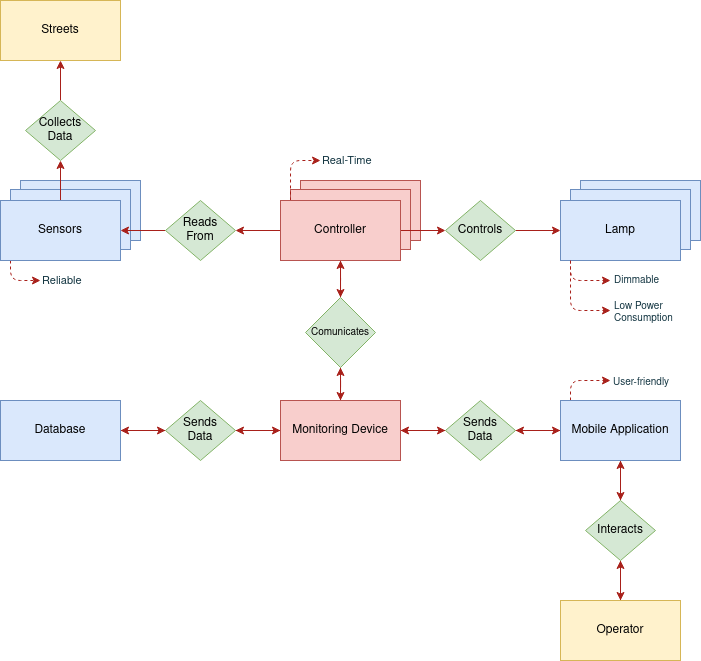
\includegraphics[width=1\textwidth]{Problem_statement_analysis}
	\caption{Problem Statement Analysis Diagram.}
	\label{fig:Problem_statement_analysis}
\end{figure}}



%When Los Angeles recently replaced more than 150,000 streetlights with LEDs, the city saved roughly 8 million dollars annually, or more than 60 percent on energy costs.
%Now, as the consequences of light pollution tiptoe from the shadows and into the spotlight, cities, regulatory agencies, and conservation groups are agitating for solutions.


\bibliographystyle{IEEEtran}
\bibliography{References}

\end{document}